\chapter{Introduction}%
\label{chap:introduction}
\textit{This chapter narrows the broad field of robotics down to a largely unsolved problem, combining the three topics; learning object dynamics, \ac{NAMO} and nonprehensile pushing. For that problem, state-of-the-art methods are presented, and their shortcomings are highlighted in the upcoming paragraphs. Then the gap in the literature regarding the combination of the aforementioned topics is summarized in \Cref{sec:research_question} in the form of the main and sub-research questions. The combination of the three topics is then narrowed down to the scope of this thesis in the problem description,~\Cref{sec:problem_description}. The chapter finishes by presenting all upcoming chapters in the report structure,~\Cref{sec:report_structure}.\bs}

For robots, navigating and acting in new, unseen environments remains a complicated problem. From the emerged challenges robots face in such environments, three topics are selected, namely: \textbf{learning object dynamics}~\cite{geist_structured_2021}, \textbf{\acf{NAMO}}~\cite{stilman_planning_2007}, and \textbf{nonprehensile pushing}~\cite{stuber_let_2020}. The main goal of this thesis is to combine these three topics. A secondary goal is to investigate how these topics can strengthen each other over time. When investigating the influence of the topics on each other, questions arise, such as: How do learned objects' system models improve global task planning for a robot with nonprehensile push manipulation abilities over time? How to combine learning and planning for push and drive applications? To what extend is the combination of the three topics; learning object dynamics, the \ac{NAMO} problem and nonprehensile pushing influenced by environmental experience? The three topics are now shortly described.\bs

Learning object dynamics enables the robot to manipulate unforeseen objects, \ac{NAMO} allows the robot to move around in an environment even if an object is blocking the robot's target location, and nonprehensile pushing allows the robot to change the environment. Combining these three topics covers any task that involves relocating objects by pushing in unforeseen robot environments, such as exploration missions or clearing debris on construction sites. An unfamiliar environment may emerge by changing a familiar environment, such as a supermarket with the presence of people. Learning abilities are crucial when the robot can encounter many different objects.\\
\acl{NAMO} can be described as; the robot having to navigate to a goal pose in an unknown environment that consists of static and movable objects. The robot may move objects if the goal can not be reached otherwise or if moving the object may significantly shorten the path to the goal~\cite{hai-ningwu_navigation_2010}.\\
Nonprehensile pushing is a form of manipulation widely available for robots, even if they are not intentionally designed for pushing. Mobile robots can drive (and thus push) against objects, and a robot arm with a gripper can push against objects even if the gripper is already full. Many robots can push, a manipulation action many robots should leverage.\\
The \ac{NAMO} problem and nonprehensile pushing are overlapping topics because both involve object manipulation. However, a given task to relocate objects in an environment consisting of movable and unmovable objects do not fit in either of the two topics individually. Relocating objects fits the combination of the \ac{NAMO} topic and the nonprehensile pushing topic. It is conceivable that a robotic system possessing the capability to both navigate through an environment and manipulate objects holds greater utility in contrast to a robot confined solely to navigation within the robot environment.\bs

Research into approaches tackling the three topics just described can be split into two categories. The bulk falls into the category of hierarchical approaches~\cite{ellis_navigation_2022,krontiris_dealing_2015,scholz_navigation_2016,vega-brown_asymptotically_2020,wang_affordancebased_2020}. The remainder falls in category locally optimal approaches~\cite{novin_dynamic_2018,sabbaghnovin_optimal_2016,sabbaghnovin_model_2021}. Both approaches are elaborated upon later in this chapter. First, the configuration space that builds up to the composite configuration space~\cite{vega-brown_asymptotically_2020} is discussed. Then secondly, two challenges are highlighted that are related to the composite configuration space growth of dimension and the fact that the composite configuration space is piecewise-analytic.\bs

\paragraph{Configuration Space}
Planning for a single action and its relation to the configuration space is now discussed. Finding a path for a single action (such as robot driving or robot pushing) is known as a \textit{motion-} or \textit{manipulation planning problem} and is planned in configuration space. \textit{Configuration space} for an object \gls{obj} can be described as an \gls{n_dof}-dimensional space, where \gls{n_dof} is the number of degrees of freedom for that single object \gls{obj}. A point in this \gls{n_dof}-dimensional configuration space fully describes where that object is in the workspace. Then the workspace obstacles are mapped to configuration space to indicate for which configurations the object \gls{obj} is in collision with an obstacle in the workspace. The subset of configurations in configuration space for which \gls{obj} is in a collision is called \textit{obstacle space}. The remainder of obstacle space subtracted from configuration space is free space, in which the object can move freely. For every object in the environment, a configuration space can be constructed. A mathematical configuration space description can be found in \Cref{subsec:path_estimation}. When a configuration space is constructed, dedicated path planners query the configuration space to determine if a configuration lies in free or obstacle space.\bs

\paragraph{Composite Configuration Space}
Planning for an action sequence and its relation to the composite configuration space is now investigated. For a robot environment that involves relocating objects among the presence of other movable objects, planning for a single action is not enough because manipulating an object directly to a target pose is often unfeasible. For example, manipulating an object $\gls{obj}_A$ to a target pose is feasible if the object $\gls{obj}_B$ that blocks that path is first removed. Clearly, removing blocking object $\gls{obj}_B$ influences the feasibility of manipulating $\gls{obj}_A$ to its target pose. For planning, there must be a connection between the configuration space of $\gls{obj}_A$ and $\gls{obj}_B$, where the composite configuration space emerges. A \textit{composite configuration space} or composite space emerges when an object's configuration space is augmented with the configuration space of other objects~\cite{vandenberg_path_2009,vega-brown_asymptotically_2020}. A composite configuration in composite space fully describes where the robot and objects are in the workspace. In recent literature, the composite configuration space is also named room configuration~\cite{sabbaghnovin_model_2021}, joint configuration space~\cite{vega-brown_asymptotically_2020} or finding \quotes{bridges} between configuration spaces~\cite{hauser_multimodal_2010}. The term composite configuration space has been adopted because it indicates multiple configuration spaces composed together. Path planners (in contrast to the planning in configuration space) have great difficulty in connecting a starting composite configuration to a target composite configuration~\cite{roynicholas_hierarchy_2021} for reasons that are discussed in the upcoming paragraph.\bs

\paragraph{Challenges}
Three challenges are now listed, two related to planning in composite space and one due to unknown environments. The first challenge is that the composite configuration space grows exponentially with the number of movable objects in the environment. The dimension of a robot environment's composite configuration space can be written as:

\[ \gls{n_obj}_\mathit{composite}^\mathit{env} = \sum_{\gls{obj} \in \gls{Obj} |_{\gls{objectClass} = \mathit{movable}}} \gls{n_obj}^{\gls{obj}}_\mathit{configuration} \]

Thus the dimension of the composite space grows linearly with the number of objects in the robot environment, and the composite configuration space itself grows exponentially, also known as the \textit{curse of dimensionality}.\bs

The second challenge is due to constraint sets. In configuration space, a single constraint set applies, where constarints originate from kinematic-, dynamic- and/or geometrical properties of the robot and the environments. For example, the boxer robot cannot drive sideways because of the constraints that orignate from the non-holonomic properties, visualise the boxer robot in \Cref{subfig:example_boxer_robot}. The non-holonomic constraints must be respected during planning for the path planner to yield feasible paths. Only a single constraint set exists in configuration space, also called \textit{mode of dynamics}~\cite{hauser_multimodal_2010}, because configuration space relates to a single action. Dedicated path planners such as \acs{PRM}~\cite{hsu_path_1997}, \acs{PRM*}, \acs{RRT} or \acs{RRT*}~\cite{karaman_samplingbased_2011} can find paths in configuration space whilst respecting the constraint set and guarantee asymptotic optimality~\cite{karaman_samplingbased_2011}. In composite space, multiple modes of dynamics exist; the composite configuration must respect the constraints set of the mode of dynamics it resides in. These different modes of dynamics make the composite configuration space \textit{piecewise-analytic}. Path planners have great difficulty crossing the boundary from one mode of dynamics to another mode of dynamics~\cite{vega-brown_asymptotically_2020}.\bs

\Cref{chap:appendix} explains complexity classes which may help understand this paragraph better. Finding an optimal action sequence to a \ac{NAMO} and nonprehensile pushing problem requires a search in composite space. Due to the challenges described above, such a problem falls in the category of \ac{NP-hard} problems, for which we now provide a reduction. If the search for an optimal solution in composite configuration space is simplified by completely removing relocating objects to new poses from the task, a purely \ac{NAMO} problem is what remains. Suppose the problem is simplified even further by assuming that every object is an unmovable obstacle. In that case, the problem falls in the category of \ac{NP-hard} problems because a reduction exists from the piano mover's problem, which is known to be \ac{NP-hard}~\cite{reif_motion_1985}. That a simplified version is \ac{NP-hard} indicates the difficulty of finding an optimal path in composite configuration space.\bs

The last challenge introduced is the uncertainty of actions in unknown environments. Planning an action sequence with limited or no environmental knowledge inevitably leads to unfeasible action sequences, such as pushing unmovable obstacles. Updating the environmental knowledge and replanning the action sequence is the cure to the uncertainty introduced by a lack of environmental knowledge. Trying to complete unfeasible action sequences is time and resources lost. Additionally, it can lead to the task itself becoming unfeasible. For example, a pushing robot pushes an object into a dead end due to an action sequence planned with limited environmental knowledge. Now that the object is stuck, the task has become unfeasible.\bs

% What is Purpose: multiple modes of dynamics, piecewise analytic
The search for an \textit{optimal} solution in composite space is unthinkable; no recent literature actually plans directly into composite space. Significant simplifications are applied to a search in the composite space, which will be discussed in the next paragraph. Finding paths for multiple actions without opting for an optimal solution, also known as multi-model planning~\cite{hauser_multimodal_2010}, can be achieved using one of the two methods. The first method connects multiple configuration spaces, \textit{hierarchical approaches}, and the second method introduces simplifications to the composite configuration space that allow finding a path, \textit{locally optimal approaches}.\bs

To summarize, the main challenge is to \textit{find an action sequence for a given task to relocate objects that consist of push and drive actions in new and unforeseen environments}. For two reasons, a search cannot be performed in the composite configuration space because it would require solving an \ac{NP-hard} problem. First, the composite space grows exponentially with the number of movable objects. Secondly, the composite configuration space piecewise-analytic path planners have great difficulty crossing boundaries from one dynamical mode to another. A multi-modal planning algorithm is sought to robustly find paths in composite configuration space whilst avoiding the emerging challenges with composite space and handling the uncertainty introduced by the lack of environmental knowledge. Several researchers tackled this problem. In the following, we provide a categorization and a summary of the most relevant state-of-the-art methods, advantages and disadvantages.\bs

\paragraph{Locally Optimal Approaches}
As indicated in the previous paragraph, finding a path in the composite configuration space cannot computationally be found in a reasonable time (orders of magnitude slower than real-time, with no guarantees if no path exists). Only by leveraging simplifications applied to the composite configuration space can a search be performed, such as considering a heavily simplified probabilistic environment~\cite{vandenberg_path_2009}, considering a single manipulation action~\cite{berenson_manipulation_2009}, discretization~\cite{sabbaghnovin_optimal_2016} or a heuristic function combined with a time horizon~\cite{sabbaghnovin_optimal_2016}. Such techniques prevent searching in configurations relatively far from the current configuration. Local optimality guarantees can be given, and real-time implementations have been shown.\bs

The most relevant locally optimal approach is presented by \citeauthor{sabbaghnovin_model_2021}. She presents an optimal motion planner~\cite{sabbaghnovin_optimal_2016} and applies it to a robot in a hospital environment~\cite{novin_dynamic_2018} to later improve upon her work~\cite{sabbaghnovin_model_2021}. The optimal motion planner avoids obstacles in the workspace and respects the kinematic and dynamic constraints of a robot arm~\cite{sabbaghnovin_optimal_2016}. Examples of the motion planner are provided using a 3- and 4- \ac{DOF} planar robot arm. Sampling in the composite configuration space is simplified using discretization (by disjunctive programming~\cite{_disjunctive_2018}) of the composite configuration space and by using a receding horizon. The disjunctive programming concept is applied to convert the continuous problem of path planning into a discrete form. In other words, a continuous path is made equivalent to some points with equal time distances representing the entire path. After discretization, the composite configuration space remains untraceable. Thus a search is performed close to the current configuration by combining a heuristic function with a receding horizon concept. A specially developed heuristic function points \textit{toward} a target configuration. The planner then plans between the current configuration and a point toward the target configuration for a predetermined time horizon. The concept of a receding horizon is used to obtain the optimal path for every time step in the time horizon, but apply only the first term and repeating this process until the end-effector meets the final pose.\bs

The optimal motion planner~\cite{sabbaghnovin_optimal_2016} is then converted toward path planning for a non-holonomic mobile robot with a gripper~\cite{novin_dynamic_2018}. With the 3-fingered gripper, the robot can grasp legged objects such as chairs or walkers. The targeted workspace is a hospital where the robot is tasked with handing walkers (or other legged objects) to patients to lower the number of falling patients. The variety of legged objects motivates an object model learning module that learns dynamic parameters from experimental data with legged objects. The dynamic parameters are learned using a Bayesian regression model~\cite{scholz_navigation_2016}. An \ac{MPC} controller then tracks the path and compensates for modelling errors. An essential contribution is that the planner can decide to re-grasp one of the object's legs to improve path tracking.\bs

Real-world experiments show the effectiveness of Novin's locally optimal approach~\cite{sabbaghnovin_model_2021}. She has presented a manipulation planning framework focused on moving legged objects in which the robot must choose which leg to push or pull. The framework can operate in real-time, and the local optimality has been shown. From the three topics this thesis focuses on, \citeauthor{sabbaghnovin_model_2021} includes learning object dynamics and prehensile manipulation of objects to target poses, missing only the \ac{NAMO} problem because a path is assumed to be free during object manipulation. Because Novin uses a gripper to manipulate objects, her research falls into the category of prehensile manipulation. Nonprehensile manipulation bears an additional challenge over prehensile manipulation. With prehensile manipulation, a gripper ensured multiple contact points, geometrically locking the object with respect to the gripper. Until the gripper opens, the gripper and gripped object can be considered a unified object. Nonprehensile manipulation, unlike prehensile manipulation, does not have the advantage of locking the object in place, making it more challenging.\bs

\paragraph{Hierarchical Approaches}
The second class of approaches to finding a path in composite configuration space is classified as hierarchical approaches~\cite{ellis_navigation_2022,krontiris_dealing_2015,scholz_navigation_2016,vega-brown_asymptotically_2020,wang_affordancebased_2020} that can be described as follows. A hierarchical structure generally consists of a high-level and a low-level component. The high-level task planner has an extended time horizon, including several atomic actions and their sequencing. Whilst a low-level controller acts to complete a single action in a single mode of dynamics, e.g.~drive toward the object, push object. The high-level planner has a prediction horizon consisting of an action sequence, a long prediction horizon compared to the low-level planner, whose prediction horizon is, at most, a single action.\bs

The most relevant hierarchical approach is presented by \citeauthor{scholz_navigation_2016}~\cite{scholz_navigation_2016}. He presents a planner for the \ac{NAMO} problem that can handle environments with under-specified object dynamics. The robot's workspace is split into various regions where the robot can move freely. Such regions can be connected if an object separates two regions and can be manipulated by the robot to connect both regions. The manipulation action is uncertain because objects have constraints that the robot has to learn, e.g.~a table has a leg that only rotates but cannot translate. A \ac{MDP} is chosen as a graph-based structure, where the nodes represent a free space region and objects separating the regions are edges in the \ac{MDP}. Finding a solution for the \ac{MDP} leads to an action sequence consisting of some drive and object manipulation actions to eventually drive the robot toward a target pose. The under-specified object dynamics introduce uncertainty in object manipulation. During action execution, object constraints are captured with a physics-based reinforcement learning framework that results in improving manipulation planning when replanning is triggered.\bs

\citeauthor{scholz_navigation_2016} presented a \ac{NAMO} planner that makes use of a hierarchical \ac{MDP} combined with a learning framework, resulting in online learning of the under-specified object dynamics. An implementation on a real robot has shown the method's effectiveness in learning and driving toward a target location. From the three topics this thesis focuses on, \citeauthor{scholz_navigation_2016} includes learning and the \ac{NAMO} problem, missing only push manipulation toward target locations. By not including manipulating objects to target poses \citeauthor{scholz_navigation_2016} can find a global path without running into high dimensional spaces. In other words, by driving only the robot toward a target location, a global path will encounter objects only once. By running into objects only once, manipulating an object does not affect the feasibility of the global path, hence the simplification.\bs


Individually a considerable amount of research is done on these three topics (learning object dynamics~\cite{cong_selfadapting_2020,seegmiller_vehicle_2013}, \ac{NAMO}~\cite{chen_fast_2018,elbanhawi_samplingbased_2014,ellis_navigation_2022,kingston_samplingbased_2018,lavalle_planning_2006,wang_affordancebased_2020}, nonprehensile pushing~\cite{arruda_uncertainty_2017,bauza_dataefficient_2018,mericli_pushmanipulation_2015,stuber_featurebased_2018,stuber_let_2020,toussaint_sequenceofconstraints_2022}). Combining two topics received little attention from the scientific community, and combining all three topics (to the best of my search) not at all. The most relevant work for local optimal~\cite{sabbaghnovin_model_2021} and hierarchical~\cite{scholz_navigation_2016} approaches are discussed, both having advantages and disadvantages. Local optimal approaches converge to a local optimal plan. To avoid the curse of dimensionality, simplifications must be used to sample the composite configuration space to be computationally feasible. Such simplifications determine the quality of solutions found. Hierarchical structures generally provide computationally efficient solutions but are hierarchical, meaning the solutions found are the best feasible solutions in the task hierarchy they search. The quality of the solution depends on the hierarchy, which is typically hand-coded and domain-specific~\cite{vega-brown_asymptotically_2020}. \Cref{table:sota_and_3_topics} presents state-of-the-art literature and which portion of the three topics they include in their research. Note that both relevant works focus on prehensile manipulation, whilst this thesis focuses on nonprehensile push manipulation. This thesis combines the three topics partly indicated in the table below by \xmark/\cmark~because learning object dynamics is only theoretically included and is not tested properly.\bs

\noindent
\begin{table}[H]
\caption{Overview of state-of-the-art literature with an indication of which topics they incorporate from the three topics; learning object dynamics, the \ac{NAMO} problem and specifying object target poses.}%
\label{table:sota_and_3_topics}
  \centering
  \rowcolors{2}{white}{myEvenLighterColor}
  \begin{tabular}
    {>{\raggedright\arraybackslash}P{2.5cm}%
      >{\raggedright\arraybackslash}P{2.0cm}%
      >{\centering\arraybackslash}P{1.4cm}%
      |>{\centering\arraybackslash}P{1.4cm}%
      >{\centering\arraybackslash}P{1.4cm}%
      |>{\centering\arraybackslash}P{1.4cm}%
      >{\centering\arraybackslash}P{1.4cm}
    }
    &&& \multicolumn{2}{c|}{\ac{NAMO}} & \multicolumn{2}{c}{\shortstack[c]{Specify object\\target poses}}\\
  Author&
  Citation&
  Learns\newline object\newline dynamics&
  \vspace{-0.2cm}\rotatebox{50}{prehensile}&
  \vspace{-0.4cm}\rotatebox{50}{nonprehesile}&
  \vspace{-0.2cm}\rotatebox{50}{prehensile}&
  \vspace{-0.4cm}\rotatebox{50}{nonprehesile}\\\hline
  \citeauthor{ellis_navigation_2022} &          \cite{ellis_navigation_2022} &          \cmark& \xmark& \cmark& \xmark& \xmark\\
  \citeauthor{sabbaghnovin_model_2021} &        \cite{sabbaghnovin_model_2021} &        \cmark& \cmark& \xmark& \cmark& \xmark\\
  \citeauthor{scholz_navigation_2016} &         \cite{scholz_navigation_2016} &         \cmark& \cmark& \xmark& \xmark& \xmark\\
  \citeauthor{vega-brown_asymptotically_2020} & \cite{vega-brown_asymptotically_2020} & \xmark& \cmark& \xmark& \cmark& \xmark\\
  \citeauthor{wang_affordancebased_2020} &      \cite{wang_affordancebased_2020} & \cmark& \xmark& \cmark& \xmark& \xmark\\
  Groote & Proposed Framework & \xmark/\cmark& \xmark& \cmark& \xmark& \cmark
\end{tabular}
\end{table}

\section{Research Question}%
\label{sec:research_question}
The following research questions have been selected to investigate the effect of learning on action selection and action planning.\bs

\textbf{Main research question:}
\begin{center}%
\label{researchquestion:main}
\large
How do learned objects' system models improve global task planning\\for a robot with nonprehensile push manipulation abilities over time?
\end{center}

The main research question is split into two smaller, more detailed subquestions.\bs

\textbf{Research subquestion:}
\begin{enumerate}
    \item\label{researchsubquestion:does_it_work} How to combine learning and planning for push and drive applications?
    \item\label{researchsubquestion:does_it_remember} To what extend is the combination of the three topics; learning object dynamics, the \ac{NAMO} problem and nonprehensile pushing influenced by environmental experience?
    \item\label{researchsubquestion:does_it_compare} How does the proposed framework compare against the state-of-the-art?
\end{enumerate}

\textbf{This thesis's main contribution is combining all three topics.} These topics are learning object dynamics, the \ac{NAMO} problem and nonprehensile push manipulation. The proposed framework combines these three topics with the \textit{\acl{halgorithm}}. The algorithm builds a graph-based structure with nodes and edges, named the \textit{\acl{hgraph}}. Planning directly in the composite configuration space is avoided due to the inherent complexity associated with planning in composite space. Instead, the \acl{halgorithm} plans only in a single mode of dynamics and searches for a global path with a technique known as a backward search~\cite{krontiris_dealing_2015}. Learned object dynamics are stored in a knowledge base called the \textit{\acl{kgraph}}. The \acl{halgorithm}, \acl{hgraph} and \acl{kgraph} are introduced in \Cref{chap:hgraph_and_kgraph}.\bs

\section{Problem Description}%
\label{sec:problem_description}
To help answer the research questions, tests are performed in a robot environment. A simple environment is desired because that simplifies testing, yet the robot environment should represent many real-world environments in which robots operate. Thus a 3-dimensional environment is selected. The environment consists of a flat ground plane since many mobile robots operate in a workspace with a flat floor, such as a supermarket, warehouse or distribution center. An environment with a flat floor and a flat robot can be treated as a 2-dimensional problem because the robot and objects can only change position over \gls{x} and \gls{y} axis ($xy$ plane parallel to the ground plane) and rotate around the $z$ axis (perpendicular to the ground plane). A flat robot is selected because it has a low center of gravity, which lowers the chance of tipping over.\bs

Let us start with defining the environment. Let the tuple $\left\langle \gls{origin}, \gls{groundPlane}, \gls{Obj}, \gls{motionEquations} \right\rangle$ fully define a robot environment where:\bs

\noindent
\begin{table}[H]
\centering
\begin{tabular}
  {>{\raggedleft\arraybackslash}p{0.13\textwidth}%
  >{\raggedright\arraybackslash}p{0.77\textwidth}}
\gls{origin}& Static point in the environment with a $x$-, $y$- and $z$-axis. Any point in the environment has a linear and an angular position and velocity with respect to the origin \vspace{0.5\baselineskip}\\
\gls{groundPlane}& A flat plane parallel with the Origin's $x$- and $y$- axis. Objects cannot pass through the ground plane and meet sliding friction when sliding over the ground plane. \vspace{0.5\baselineskip}\\
\gls{Obj}& A set of objects, $\gls{Obj} = (ob_1, ob_2, ob_3, \dots, ob_i)$ with $i\geq1$, an object is a 3-dimensional body with shape, can be unmovable or movable. In the latter case, the mass is uniformly distributed. The robot itself is considered an object, and an environment thus contains one or more objects. Examples of objects are given in \Cref{fig:example_objects}. \vspace{0.5\baselineskip}\\
\gls{motionEquations}& A set of motion equations describing the behaviour of objects. \vspace{0.5\baselineskip}\\
\end{tabular}
\end{table}

A configuration consists of the linear position of an object's center of mass with respect to the environment's origin and the angular position of an object's orientation with respect to the environment's origin.\bs

Formally, a \textbf{configuration}, $c_{id}(k)$ is a tuple of $\left\langle pos_x(k), pos_y(k), pos_\theta(k)\right\rangle$ \quad where $pos_x, pos_y \in \mathbb{R}, \quad  pos_\theta \in [0, 2\pi)$ 

$k$ indicates the time step and can be dropped to simplify the notation, \textit{id} is short for identifier and indicates the object to which this configuration belongs.\\

\subsection{Task Specification}%
\label{subsec:task}
To answer the research questions, some tasks are designed, which are defined as a subset of all objects with an associated target configuration.\bs

\[\text{task} = \left\langle \gls{Obj}_{task}, C_{targets} \right\rangle\]


Where $\gls{Obj}_{task} \subseteq \gls{Obj}$, $C_{target} = (c_1, c_2, c_3, \dots c_k)$ and $k>0$.\bs

A task is completed when the robot manages to push every object to its target configuration within a specified error margin.

\subsection{Assumptions}%
\label{subsec:assumptions}
Several assumptions are taken to simplify the pushing and learning problem, which are listed below.\bs

\noindent
\centerline{\begin{minipage}{0.9\textwidth}
\begin{assumption*}%
\label{assumption:closed_world}
\textbf{Closed-World:} Objects are manipulated, directly or indirectly, only by the robot. Influences from outside the environment cannot manipulate objects.
\end{assumption*}\bs

\begin{assumption*}%
\label{assumption:perfect_object_sensor}
\textbf{Perfect Object Sensor:} The robot has full access to the poses and geometry of all objects in the environment at all times.
\end{assumption*}\bs

\begin{assumption*}%
\label{assumption:order_does_not_matter}
\textbf{Tasks are Commutative:} Tasks consist of multiple objects with specified target poses. The order in which objects are pushed toward their target pose is commutative.
\end{assumption*}\bs

\begin{assumption*}%
\label{assumption:no_tipping}
\textbf{3-dimensional robot environment can be represented as 2-dimensional environment} All objects in the environment can be projected onto the ground plane.
\end{assumption*}\bs
\end{minipage}}

The assumptions taken serve to simplify the problem of task completion. Note that insight is given to remove all assumptions in \Cref{chap:future_work}. By removing assumptions completing tasks becomes a more complicated problem but a more realistic problem closer to real-world applications.\bs

Assumptions might have certain implications, which are listed below. The \hyperref[assumption:closed_world]{\textbf{closed-world assumption}} implies that objects that stand still and do not interact with the robot remain at the same pose. Completed subtasks are therefore assumed to be completed for all times after completion time.\bs

The \hyperref[assumption:perfect_object_sensor]{\textbf{perfect object sensor assumption}} simplifies a sensor setup, it prevents Lidar-, camera setups and tracking setups with aruco or other motion capture markers. The existence of a single perfect measurement erases the need to combine measurements from multiple sources with sensor fusion algorithms, such as Kalman filtering~\cite{verhaegen_filtering_2007}.\bs

Certain tasks are only feasible if performed in a specific order (e.g.~the Tower of Hanoi). The \hyperref[assumption:order_does_not_matter]{\textbf{tasks are commutative assumption}} allows focusing only on a single subtask since it does not affect the completion or feasibility of other subtasks.\bs

The \hyperref[assumption:no_tipping]{\textbf{3-dimensional world can be represented as 2-dimensional}} ensures that the objects in the environment can be projected onto the ground plane. Additionally, it ensures that objects do not tip over. In practice, objects will not be higher than the minimum width of the object. This experimental strategy seemed sufficient whilst running experiments but does not guarantee that objects cannot tip over.

\subsection{An Example of Robots and Objects}
To get a sense of what the robots and the objects look like, see the two robots used during testing in \Cref{fig:example_robots} as well as two example objects displayed in \Cref{fig:example_objects}.

\begin{figure}[H]
    \centering
    \begin{subfigure}{.5\textwidth}
    \centering
    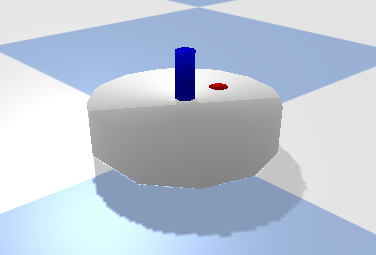
\includegraphics[width=0.9\textwidth]{figures/introduction/point_robot.png}
    \caption{The holonomic point robot with velocity input in \\\gls{x} and in \gls{y} direction}%
    \label{subfig:example_point_robot}
    \end{subfigure}%
    \begin{subfigure}{.5\textwidth}
    \centering
    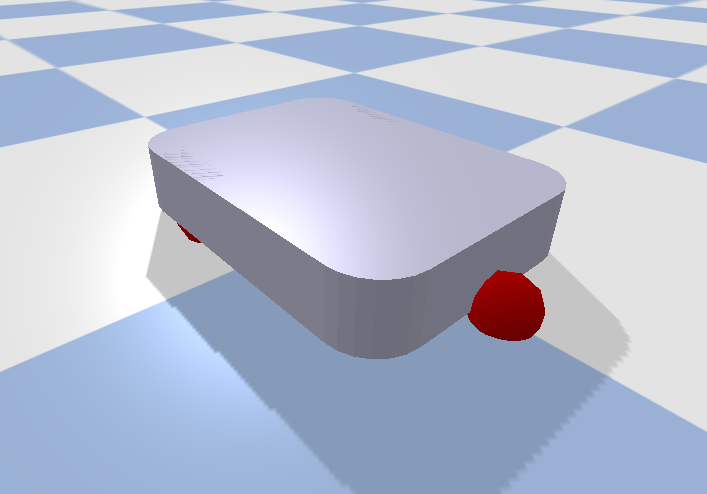
\includegraphics[width=0.85\textwidth]{figures/introduction/boxer_robot.png}
    \caption{The non-holonomic boxer robot, the\\input is forward and rotational velocity}%
    \label{subfig:example_boxer_robot}
    \end{subfigure}%
    \caption{Two robots in the robot environment}%
    \label{fig:example_robots}
\end{figure}

\begin{figure}[H]
    \centering
    \begin{subfigure}{.5\textwidth}
    \centering
    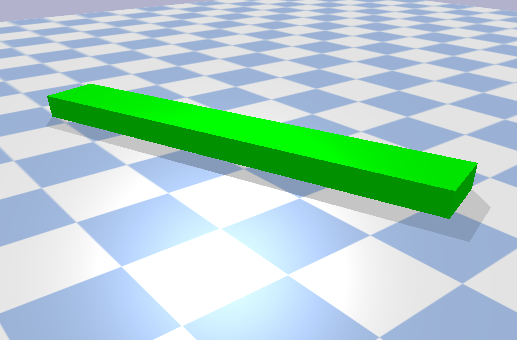
\includegraphics[width=0.9\textwidth]{figures/introduction/box_object.png}
    \caption{A box object}
    \end{subfigure}%
    \begin{subfigure}{.5\textwidth}
    \centering
    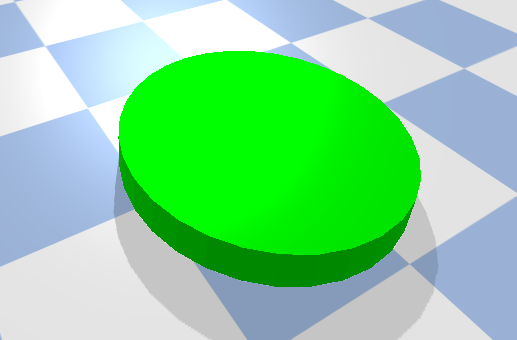
\includegraphics[width=0.9\textwidth]{figures/introduction/cylinder_object.png}
    \caption{A cylinder object}
    \end{subfigure}%
    \caption{Two objects in the robot environment}%
    \label{fig:example_objects}
\end{figure}

For complete environments with accompanying tasks, see~\Cref{chap:results}.\bs

\section{Report Structure}%
\label{sec:report_structure}
The proposed framework heavily relies on a number of methods and functions. This required background is conveniently grouped in \Cref{chap:required_background}. Then an extension is made on an existing planning algorithm in \Cref{chap:proposed_planning} to be integrated into the proposed framework that is presented and discussed in \Cref{chap:hgraph_and_kgraph}. Testing the proposed framework is presented in \Cref{chap:results}, and allows to draw conclusions in \Cref{chap:conclusion}. The last two chapters dedicate themselves to the future work and the appendix.\bs
